\subsection{Differential Contribution and Intersection}
\label{sec:ip-overlap}

%It is often useful to know whether a potential new feed contributes any new indicators relative to what a \ti\ consumer has already.
The differential contribution metric measures the number of indicators in one feed that are not in another. Equivalently, we can consider the intersection of two feeds, which is the number of elements in one feed that are present in the other, normalized by the size of the first: $|A\cap B|/|A|$. Figure~\ref{fig:overall_heatmap} shows the intersection relationship of all feeds in the study. Each cell in the matrix represents the number of elements in both feeds, normalized by the size of the feed spanning the rows on the table. That is, $A$, in the expression above, ranges over rows, and $B$ over columns of the matrix. Darker (more saturated) colors indicate greater intersection. Comparisons of feeds within a category are shaded red and comparisons of feeds between different categories are shaded blue. Note that the matrix is asymmetric, because, in general, $|A\cap B|/|A| \neq |A\cap B|/|B|$. Elements of the matrix are in the same order as in Table~\ref{tab:volume-overview-1}.

\begin{figure}
\centering
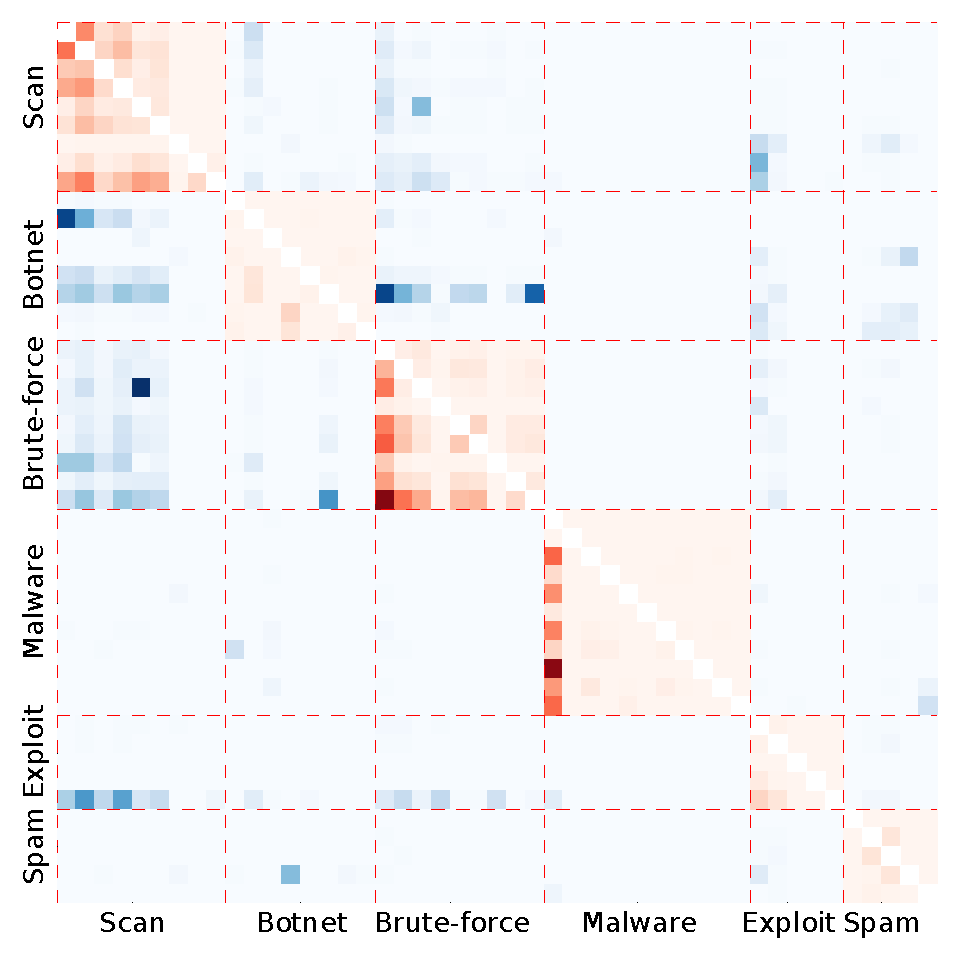
\includegraphics[width=0.475\textwidth]{images/overall_heatmap.pdf}
\caption{Feed intersection for all IP feeds. Each row/column represents a feed, shown in the same order as Table~\ref{tab:volume-overview-1}. Darker (more saturated) colors indicate greater intersection.}
\label{fig:overall_heatmap}
\end{figure}

%\begin{figure}
%\centering
%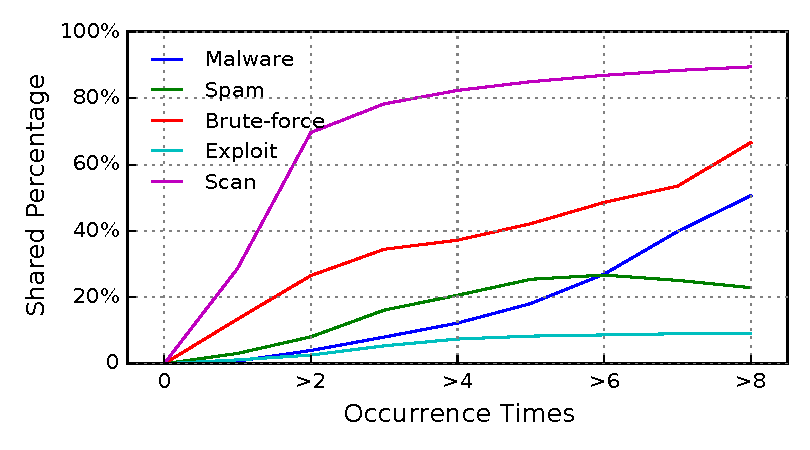
\includegraphics[width=0.4\textwidth]{images/occur_vs_overlap.pdf}
%\caption{Relation between indicators' occurrence frequency and the percentage of being shared. Each point on a line means: For the %indicators that had occurred >\emph{x} times in a feed(\textbf{X} axis), how much percent of them are shared among at least two feeds within its category(\textbf{Y} axis).}
%\label{fig:occur_vs_overlap}
%\end{figure}

\finding\ Feeds in scan and brute-force categories have higher pairwise intersections: Half of the pairwise intersection rates in two categories are greater than 5\%. The scan category has 29 out of 72 pairs (excluding self comparisons) with an intersection rate larger than 10\%, and the same case occurred in 19 out of 72 pairs in the brute-force category.

On the other side, feeds in the botnet, exploit, malware and spam category do not share much data between each other: all 4 categories have more than three-quarters of pairwise intersection rates less than 1\%. A few big feeds in these categories can share a significant amount of data with some small feeds in the same category---a characteristic that appears as a dark vertical line within its category in Figure~\ref{fig:overall_heatmap}. \feedetiprep\ in the malware category, for example, shares over 30\% of 6 other malware feeds. But the intersections among the vast majority of feeds in these 4 categories are low. This finding is consistent with prior work~\cite{metcalf2015blacklist,thomas2016abuse}, but we provide a more comprehensive view regarding different categories.

Figure~\ref{fig:overall_heatmap} also shows the relation between feeds across different categories. We can clearly see a relation between scan and brute-force feeds: multiple scan feeds have non-trivial intersection with feeds in the brute-force category. In fact, 23.1\% of all 760,263 brute-force IPs we collected are also included by scan feeds in our dataset. There are also three botnet feeds---\feedTSCI, \feedTSVoIP\ and \feedTSCompr---that have over 10\% of its data shared with multiple feeds in the scan category.

%\noteby{KL}{Cut this paragraph and accompanying figure.}
%One interesting question is: Are indicators that occurred multiple times in a feed more likely to be shared between feeds? We check this question by calculating how much percent of indicators, that had occurred more than \emph{x} times in a feed, are shared between at least two feeds within each category. The result is shown in Figure~\ref{fig:occur_vs_overlap}. Botnet category is excluded from the Figure since the percentages are too low to argue about the trend. We can see that there is a strong positive correlation between the occurrence frequency and the percentage being shared, across different categories. This aligns with the intuition that a persistent attacker is more likely being observed by mulitple \ti\ sources.
